\chapter{Numerical Results}

\section{Fixed Schedule}

\section{Alterable Schedule}

\subsection{State (3, 2)}

Assume that the mean service time $\mu$ is $1$. In addition, assume that the per unit time costs of the customers' waiting time and server's idle time ($c_{W}$ and $c_{I}$ respectively) are both $1$. Under these assumptions, the cost of state $(3, 2)$ for various values of $a$ is given by the following expression, which is continuous for $a \geq 0$.

\begin{equation*}
	C_{3} (a, 2) =
	\begin{cases}
 		9.88121 & \text{where $a = 0$} \\
 		\frac{\mathrm{e}^{-a} \left( \mathrm{e}^{a} a (2.29362 - 0.5 a) - (0.5 a + 3.29362) a - 1.15888 \mathrm{e}^{a} + (a + 5.52005) \mathrm{e}^{2 a} - 4.36117 \right)}{\mathrm{e}^{a} - 1} & \text{where $a > 0$}
	\end{cases}
\end{equation*}

This equation is plotted for $a \in [0, 10]$ to visualise the relationship between the cost and $a$. The resulting figure is Figure \ref{Graph_3_2}.

\begin{figure}[htb]
	\centering
	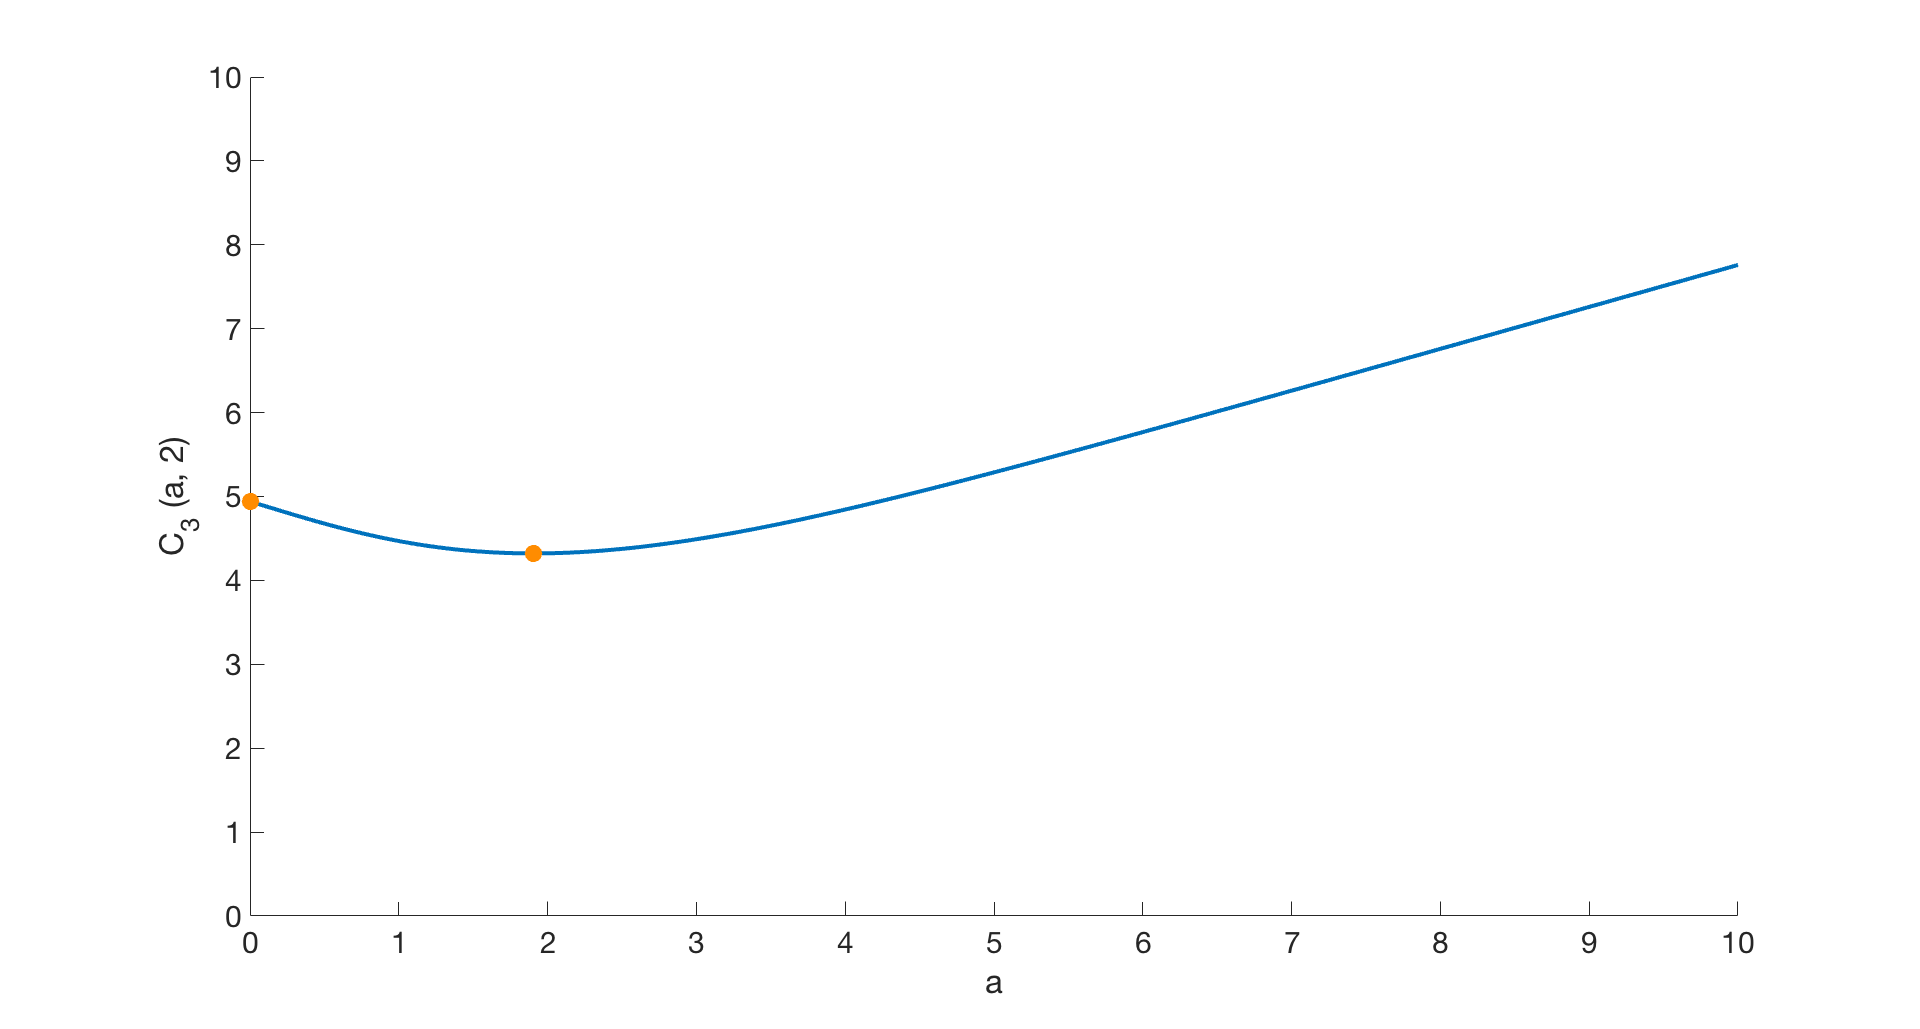
\includegraphics[width = 0.85\textwidth]{Graph_3_2.png}
	\caption{Cost of state with n = 3, k = 2 for various values of a}
	\label{Graph_3_2}
\end{figure}

The only value of $a$ where $\frac{\partial}{\partial a} C_{3} (a, 2) = 0$ is $1.90481$. Thus, the set of possible policies $\mathcal{A}$ is $\{ 0, 1.90481 \}$ whereby there are two possible policies labelled as orange dots on Figure \ref{Graph_3_2}. Moreover, note that as $a$ increases beyond 2, the cost increases approximately linearly as the expected waiting time of the next customer and the expected idle time of the server both increase linearly.

The optimal policy $a^{*}$ that minimises $C_{3} (a, 2)$ is $1.90481$ where the cost is $8.64338$. If on arrival of a customer, there are $2$ customers in the queue and $3$ customers remaining to be scheduled, then the next customer should be scheduled to arrive in $1.90481$ time units. This is slightly below the expected service time of the two customers in the queue to account for the idle cost of the server.

\subsection{6 Customers}

Assume there are 6 customers that need to be scheduled for service who all have a mean service time $\mu$ of 1. The initial state is $(6, 0)$, and the possible states during service are all states in the set

\begin{equation}
	\Big\{ (n, k) \in \{ 0, 1, \ldots, 6 \}^{2} : n + k \leq 6 \Big\}
\end{equation}

\begin{table}[htb]
	\centering
	\begin{tabular}{c c c || c | c | c | c | c | c | c}
		& & & \multicolumn{7}{c}{queue length ($k$)} \\
		& & & 0 & 1 & 2 & 3 & 4 & 5 & 6 \\ \hline \hline
		\parbox[t]{2mm}{\multirow{7}{*}{\rotatebox[origin=c]{90}{customers to be}}} & \parbox[t]{2mm}{\multirow{7}{*}{\rotatebox[origin=c]{90}{scheduled ($n$)}}} & 0 & 0 & 1 & 3 & 6 & 10 & 15 & 21 \\
		& & 1 & 1 & 2.69315 & 4.97937 & 8.04949 & 11.9605 & 16.7418 \\
		& & 2 & 2.69315 & 4.52005 & 6.81367 & 9.88121 & 13.7875 & \\
		& & 3 & 4.52005 & 6.35018 & 8.64338 & 11.7105 & & \\
		& & 4 & 6.35018 & 8.18013 & 10.4733 & & & \\
		& & 5 & 8.18013 & 10.0101 & & & & \\
		& & 6 & 10.0101 & & & & & \\
	\end{tabular}
	\caption{Cost of possible states for 6 total customers}
	\label{Cost_6_Customers}
\end{table}

Table \ref{Cost_6_Customers} displays the calculated expected costs for each possible state if there are 6 total customers (assuming $c_{W} = c_{I} = 1$). The cost of the initial state is $10.0101$, thus the expected cost of servicing six customers with an alterable schedule is $10.0101$.

Note that in this table, for $n \geq 1$, $C_{n}^{*} (0) = C_{n - 1}^{*} (1)$. This is due to the fact that if there are no customers currently waiting (e.g., initially), then it is always optimal to schedule the next arrival immediately. The expected cost thus doesn't change as the next arrival occurs immediately.

The worst state on this table is the state $(0, 6)$, which is all six customers waiting for serviced. This can occur if all six customers are scheduled to arrive immediately (to ensure no idle time), or the first customer has an extremely long service time.

\begin{table}[htb]
	\centering
	\begin{tabular}{c c c || c | c | c | c | c | c}
		& & & \multicolumn{6}{c}{queue length ($k$)} \\
		& & & 0 & 1 & 2 & 3 & 4 & 5 \\ \hline \hline
		\parbox[t]{2mm}{\multirow{6}{*}{\rotatebox[origin=c]{90}{customers to be}}} & \parbox[t]{2mm}{\multirow{6}{*}{\rotatebox[origin=c]{90}{scheduled ($n$)}}} & 1 & 0 & 0.693147 & 1.75711 & 2.82577 & 3.85505 & 4.8492 \\
		& & 2 & 0 & 0.826902 & 1.90223 & 2.95223 & 3.95872 & \\
		& & 3 & 0 & 0.83013 & 1.90481 & 2.95403 & & \\
		& & 4 & 0 & 0.82995 & 1.90455 & & & \\
		& & 5 & 0 & 0.829925 & & & & \\
		& & 6 & 0 & & & & & \\
	\end{tabular}
	\caption{Optimal policy for each possible states for 6 total customers}
	\label{Policy_6_Customers}
\end{table}

Table \ref{Policy_6_Customers} displays the corresponding arrival times for the costs in Table \ref{Cost_6_Customers}. This table does not include any optimal times for $n = 0$, as there is no next customer to schedule in those states.

The first pattern to notice is (as discussed earlier) if there are no customers currently waiting (i.e., $k = 0$), then the optimal solution is to schedule the next arrival immediately. This makes intutive sense as scheduling the next arrival immediately minimises the future idle time and ensures that the waiting time of the next customer is simpler their service time.

As $k$ increases for constant $n$, the optimal schedule time increases approxiimately proportionately. The optimal $a^{*}$ increases by approximately $\mu$ for each extra $k$ to minimise the waiting time of the next customer.

Finally, for $n \geq 1$, the value of $a^{*}$ such that $C_{n}^{*} (k) = C_{n} (a^{*}, k)$ is always less than $\mu k$ (i.e., the expected time for the queue to be empty). This is due to the cost of the idle time of the customer leading to the desire for the next customer to arrive just before the queue becomes empty.